\documentclass[12pt, stu, floatsintext, hidelinks]{apa7}

\usepackage{graphicx}
\usepackage{threeparttable}
\usepackage{lipsum}
\usepackage{float}
\usepackage{annotate-equations}
\usepackage{mathptmx} % Times Roman font
\usepackage{xpatch}

%%% apa7 doesn't want to add appendix section titles in the toc
%%% let's make it do it
\makeatletter
\xpatchcmd{\appendix}
  {\par}
  {\addcontentsline{toc}{section}{\@currentlabelname}\par}
  {}{}
\makeatother

% Python code highlighting stuff
\usepackage{pythonhighlight}
% Python code highlighting stuff

\usepackage[style=apa]{biblatex}
\addbibresource{refs.bib}

\title{Applying Finite-Difference Equations to find Nodal Temperatures}
\author{Gregory Dsouza}
% \authorsnames{For, Multiple, Different, Authors}
\course{ES 403: Heat Transfer}
\professor{Prof. Yang Chao}
\duedate{\today}
\authorsaffiliations{Embry-Riddle Aeronautical University}

\usepackage[final]{draftwatermark} % Remove or put "final" in the options to remove the watermark

\begin{document}
\clearpage
\maketitle
\tableofcontents
\clearpage

\section{Sets of Equations}
\subsection{Interior Equations}

$$
	T_{b} + T_{10} - 4.0 T_{9} + T_{1} + T_{17} = 0
$$
$$
	- 4.0 T_{10} + T_{11} + T_{9} + T_{18} + T_{2} = 0.0
$$
$$
	T_{10} - 4.0 T_{11} + T_{12} + T_{19} + T_{3} = 0.0
$$
$$
	T_{11} - 4.0 T_{12} + T_{13} + T_{20} + T_{4} = 0.0
$$
$$
	T_{12} - 4.0 T_{13} + T_{14} + T_{21} + T_{5} = 0.0
$$
$$
	T_{13} - 4.0 T_{14} + T_{15} + T_{22} + T_{6} = 0.0
$$


\subsection{Exterior Equations with Convection}

$$
	T_{b} + 2.0 T_{9} + T_{2} + \frac{2.0 T_{\infty} \Delta{x} h}{k} = 2.0 T_{1} \left(\frac{\Delta{x} h}{k} + 2.0\right)
$$
$$
	T_{b} + 2.0 T_{9} + T_{18} + \frac{2.0 T_{\infty} \Delta{x} h}{k} = 2.0 T_{17} \left(\frac{\Delta{x} h}{k} + 2.0\right)
$$
$$
	2.0 T_{10} + T_{1} + T_{3} + \frac{2.0 T_{\infty} \Delta{x} h}{k} = 2.0 T_{2} \left(\frac{\Delta{x} h}{k} + 2.0\right)
$$
$$
	2.0 T_{10} + T_{17} + T_{19} + \frac{2.0 T_{\infty} \Delta{x} h}{k} = 2.0 T_{18} \left(\frac{\Delta{x} h}{k} + 2.0\right)
$$
$$
	2.0 T_{11} + T_{2} + T_{4} + \frac{2.0 T_{\infty} \Delta{x} h}{k} = 2.0 T_{3} \left(\frac{\Delta{x} h}{k} + 2.0\right)
$$
$$
	2.0 T_{11} + T_{18} + T_{20} + \frac{2.0 T_{\infty} \Delta{x} h}{k} = 2.0 T_{19} \left(\frac{\Delta{x} h}{k} + 2.0\right)
$$
$$
	2.0 T_{12} + T_{3} + T_{5} + \frac{2.0 T_{\infty} \Delta{x} h}{k} = 2.0 T_{4} \left(\frac{\Delta{x} h}{k} + 2.0\right)
$$
$$
	2.0 T_{12} + T_{19} + T_{21} + \frac{2.0 T_{\infty} \Delta{x} h}{k} = 2.0 T_{20} \left(\frac{\Delta{x} h}{k} + 2.0\right)
$$
$$
	2.0 T_{13} + T_{4} + T_{6} + \frac{2.0 T_{\infty} \Delta{x} h}{k} = 2.0 T_{5} \left(\frac{\Delta{x} h}{k} + 2.0\right)
$$
$$
	2.0 T_{13} + T_{20} + T_{22} + \frac{2.0 T_{\infty} \Delta{x} h}{k} = 2.0 T_{21} \left(\frac{\Delta{x} h}{k} + 2.0\right)
$$
$$
	2.0 T_{14} + T_{5} + T_{7} + \frac{2.0 T_{\infty} \Delta{x} h}{k} = 2.0 T_{6} \left(\frac{\Delta{x} h}{k} + 2.0\right)
$$
$$
	2.0 T_{14} + T_{21} + T_{23} + \frac{2.0 T_{\infty} \Delta{x} h}{k} = 2.0 T_{22} \left(\frac{\Delta{x} h}{k} + 2.0\right)
$$
$$
	2.0 T_{15} + T_{6} + T_{8} + \frac{2.0 T_{\infty} \Delta{x} h}{k} = 2.0 T_{7} \left(\frac{\Delta{x} h}{k} + 2.0\right)
$$
$$
	2.0 T_{15} + T_{22} + T_{24} + \frac{2.0 T_{\infty} \Delta{x} h}{k} = 2.0 T_{23} \left(\frac{\Delta{x} h}{k} + 2.0\right)
$$
$$
	2.0 T_{16} + 2.0 T_{7} + \frac{2.0 T_{\infty} \Delta{x} h}{k} = 2.0 T_{8} \left(\frac{\Delta{x} h}{k} + 2.0\right)
$$
$$
	2.0 T_{16} + 2.0 T_{23} + \frac{2.0 T_{\infty} \Delta{x} h}{k} = 2.0 T_{24} \left(\frac{\Delta{x} h}{k} + 2.0\right)
$$


\subsection{Exterior Equations with Insulation}

$$
	T_{14} - 4.0 T_{15} + T_{16} + T_{23} + T_{7} = 0.0
$$
$$
	2.0 T_{15} - 4.0 T_{16} + T_{24} + T_{8} = 0
$$

\section{Tabulated Temperatures and Plots}

\begin{table}[H]
	\centering
	\caption{Final Nodal Temperatures}
	\begin{threeparttable}
		\begin{tabular}{llllllll}
			\toprule
			\multicolumn{8}{c}{Temperature ($^\circ$F)}                             \\
			\midrule
			113.598 & 91.279  & 84.111 & 81.546 & 80.589 & 80.229 & 80.098 & 80.065 \\
			131.955 & 100.622 & 87.976 & 83.060 & 81.174 & 80.457 & 80.196 & 80.130 \\
			113.598 & 91.279  & 84.111 & 81.546 & 80.589 & 80.229 & 80.098 & 80.065 \\
			\bottomrule
		\end{tabular}
	\end{threeparttable}
\end{table}

\begin{figure}[H]
	\makebox[\textwidth]{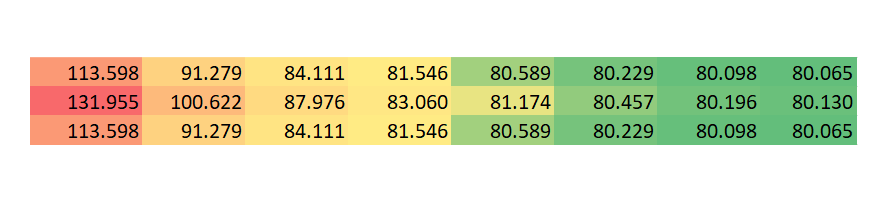
\includegraphics[width=0.8\paperwidth]{ColorPlot.png}}
	\caption{Colored Distribution of Nodal Temperatures}
\end{figure}

\section{Explanation of Software Code}

All software code used can be seen in \autoref{software-code}. I chose to use Python to prepare a script to calculate the nodal temperatures. The script relies of 3 external dependencies:

\begin{itemize}
	\item sympy
	\item xlsxwriter
	\item pandas
\end{itemize}

Two of these dependencies are commonly used well known packages. ``Sympy'' is a python module that is used to define and solve systems of equations, ``xlsxwriter'' is used to write out python data to an excel file, and ``Pandas'' is used to print the data of the excel file to the console window. These dependencies can be installed with the following commands on a Windows python distribution:

\begin{python}
pip install sympy
pip install pandas
pip install xlsxwriter
\end{python}

For this reason, I have also included a message at the beginning of the script to warn about the excel file that is generated when the script is run. We start by defining the properties of the system:

\begin{itemize}
	\item $k$, the thermal conductivity
	\item $h$, the convection heat transfer coefficient
	\item $T_{\infty}$, the temperature of the surroundings
	\item $T_b$, the base temperature
	\item $\Delta x$, the horizontal distance between each node
	\item $\Delta y$, the vertical distance between each node
\end{itemize}

I then created a generalized ``TNode'' class that holds all the information and attributes of a single temperature node, including its neighbors and its own nodal temperature.

We then create a grid of these ``TNode'' objects and iterate over the grid after it has been created to find and assign all the neighbors. After doing this, we define variables for each temperature node in the grid using Sympy.

Using this along with our new grid of ``TNodes'', we can apply our finite-difference equations by iterating over the grid and setting up a system of equations using variables from Sympy, and appending them to a list that we can pass as a linear system of equations to solve later.

This system of equations is then solved by Sympy and the solution temperatures are tabulated and output to an excel file for any further calculations that the user may wish to do with these nodal temperatures.

Lastly, the nodal temperatures are also printed to the console window using ``Pandas'' so that they can be quickly viewed.

\appendix

\section{Heat Conduction Analysis Code}
\label{software-code}

% Import code from file
\inputpython{heat_conduction_analysis.py}{1}{193}

\end{document}